% mẫu latex dùng cho đồ án 1, đồ án 2, và luận văn tốt nghiệp
% trường đại học sư phạm kỹ thuật tp hcm
% khoa điện điện tử
% bộ môn máy tính - viễn thông
% template được xây dựng lại dựa trên https://github.com/thanhhungqb/thesis-template
% mọi thắc mắc liên hệ: TS. Huỳnh Thế Thiện
\documentclass[a4paper, oneside]{book}
\usepackage[fontsize=13pt]{scrextend}
\usepackage{setspace}
\usepackage[utf8]{inputenc} 
\usepackage[T1]{fontenc} 
\usepackage[vietnamese,english]{babel} 

\usepackage[
singlelinecheck=false % <-- important
]{caption}
\usepackage{cite}
\usepackage{amsmath,amssymb,amsfonts}
\usepackage{algorithmic}
\usepackage{graphicx}
\usepackage{textcomp}
\usepackage{epsfig}
\usepackage{multirow}
\usepackage{xcolor}
\usepackage{float}
\usepackage{subfigure}
\usepackage[hidelinks]{hyperref}
\usepackage{mathptmx}
\usepackage{fancyhdr}
\usepackage{algorithm2e}
\usepackage{hmcutethesis}

% {\fontsize{20}{1}\selectfont \textbf{\parbox[c][3cm]{0.9\linewidth}{ \centering \@tname }}} \\[1cm]

\ctname{\textbf{HƯỚNG DẪN TRÌNH BÀY BÁO CÁO KHÓA LUẬN}} 
\cmjname{\textbf{NGÀNH: ĐIỆN TỬ VIỄN THÔNG - 8520208}}
\cstuname{\textbf{HỌ TÊN HỌC VIÊN}} % với nhóm 2 sinh viên
% \cstuname{\textbf{TÊN SINH VIÊN} \\[3pt] MSSV: XXXXXXXX} % với nhóm 1 sinh viên
\csSupervise{TS. NGUYỄN VĂN A}
\cttime{06/2023}



\thesislayout
\setstretch{1.5}

\begin{document}
%-	Bìa cứng - màu xanh dương, chữ mạ vàng (xem mẫu đính kèm)
%-	Trang tên (tờ lót): chất liệu giấy, nội dung giống như bìa LV
%-	Ở gáy LV: in nhan đề LV (có thể in tóm tắt nếu nhan đề quá dài), size 15 – 17
%-	Phiếu Nhiệm vụ LV, chấm điểm Hướng dẫn & Phản biện (đã ký): nhận từ GVHD & GVPB sau khi bảo vệ (theo lịch hẹn).
%-	Lời cam đoan
%-	Lời cảm ơn/ Lời ngỏ
%-	Tóm tắt LV
%-	Mục lục
%-	Danh mục, bảng biểu, hình ảnh, ... (nếu có)
%-	Nội dung LV
%-	Danh mục TL tham khảo
%-	Phụ lục (nếu có)
\coverpage
\frontmatter


% lời cảm ơn ================================================
\begin{acknowledgments}
	Trong quá trình tự mình hoàn thành đồ án môn học 1/2 (hoặc đồ án tốt nghiệp) với đề tài, tôi đã nhận được rất nhiều sự tư vấn và lời khuyên từ Thầy Cô... Tôi xin chân thành cảm ơn!
\begin{table}[!h]
\centering
\begin{tabular}{p{3cm} p{3cm} p{3cm} p{3cm}}
&  & \multicolumn{2}{c}{Nhóm thực hiện đồ án tốt nghiệp} \\
&  & \multicolumn{2}{c}{\textit{(Ký và ghi rõ họ tên)}} \\
&  &             &            \\
&  &             &            \\
&  &             &            \\
&  &             &            \\
&  &             &            \\
&  &             &            \\
&  & \multicolumn{2}{c}{Nguyễn Văn B}     
\end{tabular}
\end{table}
\end{acknowledgments}

% lời cam đoan ================================================
\begin{declaration}
	Nhóm thực hiện đồ án tốt nghiệp cam đoan đề tài thực hiện dựa vào một số tài liệu trước đó và không sao chép nội dung, kết quả của đồ án khác. Các nội dung tham khảo đã được trích dẫn đầy đủ.
 \\
\begin{table}[!h]
\centering
\begin{tabular}{p{3cm} p{3cm} p{3cm} p{3cm}}
&  & \multicolumn{2}{c}{Nhóm thực hiện đồ án tốt nghiệp} \\
&  & \multicolumn{2}{c}{\textit{(Ký và ghi rõ họ tên)}} \\
&  &             &            \\
&  &             &            \\
&  &             &            \\
&  &             &            \\
&  &             &            \\
&  &             &            \\
&  & \multicolumn{2}{c}{Nguyễn Văn B}       
\end{tabular}
\end{table}
\end{declaration}

% Tóm tắt LV ================================================
\begin{abstract}
	Tóm tắt luận văn ...
\end{abstract}	


% mục lục, danh sách bảng, danh sách hình tự động
\tableofcontents
\listoftables
\listoffigures


% danh sách các từ viết tắt =================================
\begin{abbreviation}
Dưới đây là danh mục các từ viết tắt được sử dụng trong luận văn.
\begin{table}[!h]
\renewcommand{\arraystretch}{1.3}
\begin{tabular}{p{3cm} p{11cm}}
\textbf{Các từ viết tắt} &  \textbf{Định nghĩa} \\
DL & Deep Learning \\
YOLO & You Only Look Once \\
AI & Artificial Intelligence \\
\end{tabular}
\end{table}
\end{abbreviation}	



\mainmatter


%  đánh số trang cho thesis ==================================
\fancypagestyle{plain}{
  \fancyhf{} % Clear header and footer
  \renewcommand{\headrulewidth}{0pt} % Remove header rule
  \fancyfoot[c]{\thepage} % Centered page number
}
\pagestyle{plain} % Apply the page style to all pages


% nội dung thesis được viết riêng cho từng chương (chapter)
\chapter{TỔNG QUAN}
\section{Giới thiệu}
Giới thiệu được viết tại đây ... 
\subsection{Giới thiệu về AI}
AI là ... 
\subsubsection{Giới thiệu về ML}
ML là machine learning~\cite{zhu2022}... 
\section{Mục tiêu}
Mục tiêu của đề tài ...

\section{Tình hình nghiên cứu}
Cách để trích dẫn bài báo xuất bản trong tạp chí~\cite{huynhthe2021}, bài báo được trình bài tại hội nghị~\cite{said2014biometric} và đường link của một trang web~~\cite{IoTDesignPro}

\section{Phương pháp nghiên cứu}
Để đạt được mục tiêu của đề tài, tôi sử dụng các phương pháp thu thập số liệu, thực nghiệm và phân tích tổng kết kinh nghiệm. 
\begin{itemize}
    \item Phương pháp thu thập số liệu:
    \begin{itemize}
        \item Sử dụng phương pháp quan sát: Tôi tiến hành quan sát trực ...
        \item Tiến hành cuộc phỏng vấn: Tôi tiến hành cuộc phỏng vấn ...
    \end{itemize}
    \item Phương pháp thực nghiệm: 
    \begin{itemize}
        \item Thiết kế và triển khai hệ thống: Tôi tiến hành thiết kế và triển khai ...
        \item Tiến hành thử nghiệm: Tôi thực hiện các bài kiểm tra và thử nghiệm hệ thống ...
    \end{itemize}    
    \item Phương pháp phân tích tổng kết kinh nghiệm: 
    \begin{itemize}
        \item Đánh giá hiệu quả: Tôi tiến hành đánh giá hiệu quả ...
        \item Phân tích dữ liệu: Tôi phân tích dữ liệu ...
        \item Tổng kết kinh nghiệm: Dựa trên kết quả phân tích, tôi tổng kết kinh nghiệm ...
    \end{itemize}
\end{itemize}

\section{Bố cục nội dung}
Báo cáo đồ án môn học 1 của tôi sẽ bao gồm 5 chương:
\begin{itemize}
    \item Chương 1: Tổng quan
    \item Chương 2: Cơ sở lý thuyết
    \item Chương 3: Thiết kế hệ thống
    \item Chương 4: Kết quả
    \item Chương 5: Kết luận và hướng phát triển.
\end{itemize}




% \begin{figure}[!t]
% 	\centering
% 	
\includegraphics[width=87.5mm]{hcmutelogo.png}
% 	\caption{SPWVD-TFIs of radar and communication waveform types.}
% 	\label{fig_example}
% \end{figure}

% \section{Yêu cầu và mục tiêu của đề tài}

% \subsection{Yêu cầu}

% Nghiên cứu thuật toán phân loại tin nhắn rác.

% Tạo ứng dụng chặn tin nhắn rác trên điện thoại thông minh (Android)

% \subsection{Mục tiêu}

% \subsubsection{Về kiến thức}

% Phân tích, giải quyết yêu cầu bài toán phân loại tin nhắn rác

% Nắm vững các thuật toán phân loại sử dụng

% Nắm các kỹ thuật xử lý văn bản: tách token, tính xác suất các token,\ldots

% Nắm các kiến thức lập trình di động (Android)

% \subsubsection{Về sản phẩm}

% \begin{table}[!t]
% \footnotesize
% \caption{Summary of Performance Comparison.}
% \begin{tabular}{@{}l r r r@{}}
% \hline
% \multirow{1}{*}{Networks}	& Size (params.) & Speed (ms) & Acc. ($\%$)  \\ \hline
% Lin~\textit{et al.}~\cite{lin2020unknown}	&$	1.4\mathrm{M}	$&$	0.0390	$&$	87.66	$\\
% Shen~\textit{et al.}~\cite{shen2022radar}	&$	6.1\mathrm{M}	$&$	0.0384	$&$	87.62	$\\
% % Huynh-The~\textit{et al.}~\cite{huynhthe2022racomnet}	&$	315\mathrm{K}	$&$	0.0536	$&$	89.91	$\\
% Huynh-The~\textit{et al.}~\cite{huynhthe2022racomnet}	&$	315\mathrm{K}	$&$	0.0586	$&$	89.91	$\\
% MobileNetv2~\cite{sandler2018mobilenetv2}	&$	2.2\mathrm{M}	$&$	0.0621	$&$	87.92	$\\
% ResNet50~\cite{he2016deep}	&$	23.5\mathrm{M}	$&$	0.0683	$&$	87.34	$\\
% Inception-V3~\cite{szegedy2016inception}	&$	21.8\mathrm{M}	$&$	0.1059	$&$	89.94	$\\
% EfficientNetb0~\cite{tan2019efficientnet}	&$	4.0\mathrm{M}	$&$	0.0823	$&$	89.47	$\\ 
% Sim-RadComNet	&$	180\mathrm{K}		$&$	0.1055	$&$	87.46	$\\
% Reg-RadComNet	&$	6.1\mathrm{M}		$&$	0.1270	$&$	89.47	$\\ \hline
% RadComNet ($2$ RSA modules)	&$	102\mathrm{K}		$&$	0.0602	$&$	82.85	$\\
% RadComNet ($3$ RSA modules)	&$	140\mathrm{K}		$&$	0.0644	$&$	86.85	$\\
% RadComNet ($4$ RSA modules)	&$	178\mathrm{K}		$&$	0.0679	$&$	89.87	$\\
% RadComNet ($5$ RSA modules)	&$	216\mathrm{K}		$&$	0.0712	$&$	90.56	$\\
% RadComNet ($6$ RSA modules)	&$	254\mathrm{K}		$&$	0.0744	$&$	90.89	$\\
% \hline
% \end{tabular}
% \label{tab_compare}
% \end{table}

% Tối ưu hóa bộ lọc, ứng dụng

% Nắm được quy trình phát triển sản phẩm: phân tích - thiết kế - hiện thực - kiểm tra.

% Phát triển ứng dụng thực tế, hướng sử dụng, tương tác.

% \section{Bố cục của luận văn}




\chapter{CƠ SỞ LÝ THUYẾT}
\section{Bảng và hình}
\subsection{Bảng}
Cách trình bày bảng~\ref{tab01} ... 

\begin{table}[!h]
\footnotesize
\caption{Bảng so sánh hiệu năng.}
\begin{tabular}{@{}l r r r@{}}
\hline
\multirow{1}{*}{Networks}	& Size (params.) & Speed (ms) & Acc. ($\%$)  \\ \hline
Method 1 &$	1.4\mathrm{M}	$&$	0.0390	$&$	87.66	$\\
Method 2	&$	6.1\mathrm{M}	$&$	0.0384	$&$	87.62	$\\
Method 3 &$	315\mathrm{K}	$&$	0.0586	$&$	89.91	$\\
MobileNetv2&$	2.2\mathrm{M}	$&$	0.0621	$&$	87.92	$\\
ResNet50&$	23.5\mathrm{M}	$&$	0.0683	$&$	87.34	$\\
Inception-V3&$	21.8\mathrm{M}	$&$	0.1059	$&$	89.94	$\\
EfficientNetb0&$	4.0\mathrm{M}	$&$	0.0823	$&$	89.47	$\\ 
Sim-RadComNet	&$	180\mathrm{K}		$&$	0.1055	$&$	87.46	$\\
Reg-RadComNet	&$	6.1\mathrm{M}		$&$	0.1270	$&$	89.47	$\\ \hline
RadComNet ($2$ RSA modules)	&$	102\mathrm{K}		$&$	0.0602	$&$	82.85	$\\
RadComNet ($3$ RSA modules)	&$	140\mathrm{K}		$&$	0.0644	$&$	86.85	$\\
RadComNet ($4$ RSA modules)	&$	178\mathrm{K}		$&$	0.0679	$&$	89.87	$\\
RadComNet ($5$ RSA modules)	&$	216\mathrm{K}		$&$	0.0712	$&$	90.56	$\\
RadComNet ($6$ RSA modules)	&$	254\mathrm{K}		$&$	0.0744	$&$	90.89	$\\
\hline
\end{tabular}
\label{tab01}
\end{table}

\begin{table}[!h]
\caption{Bảng điểm sinh viên}
\begin{tabular}{llll}
\hline
\multicolumn{1}{c}{MSSV} & \multicolumn{1}{c}{Họ} & \multicolumn{1}{c}{Tên} & \multicolumn{1}{c}{Điểm} \\ \hline
                         &                        & A                       & \multirow{2}{*}{8}       \\
                         &                        & B                       &                          \\
                         &                        &                         &                         
\end{tabular}
\label{tab02}
\end{table}

\subsection{Hình}
Hình được trình bày và tham khảo đến hình~\ref{fig01}...

\begin{figure}[!t]
	\centering
	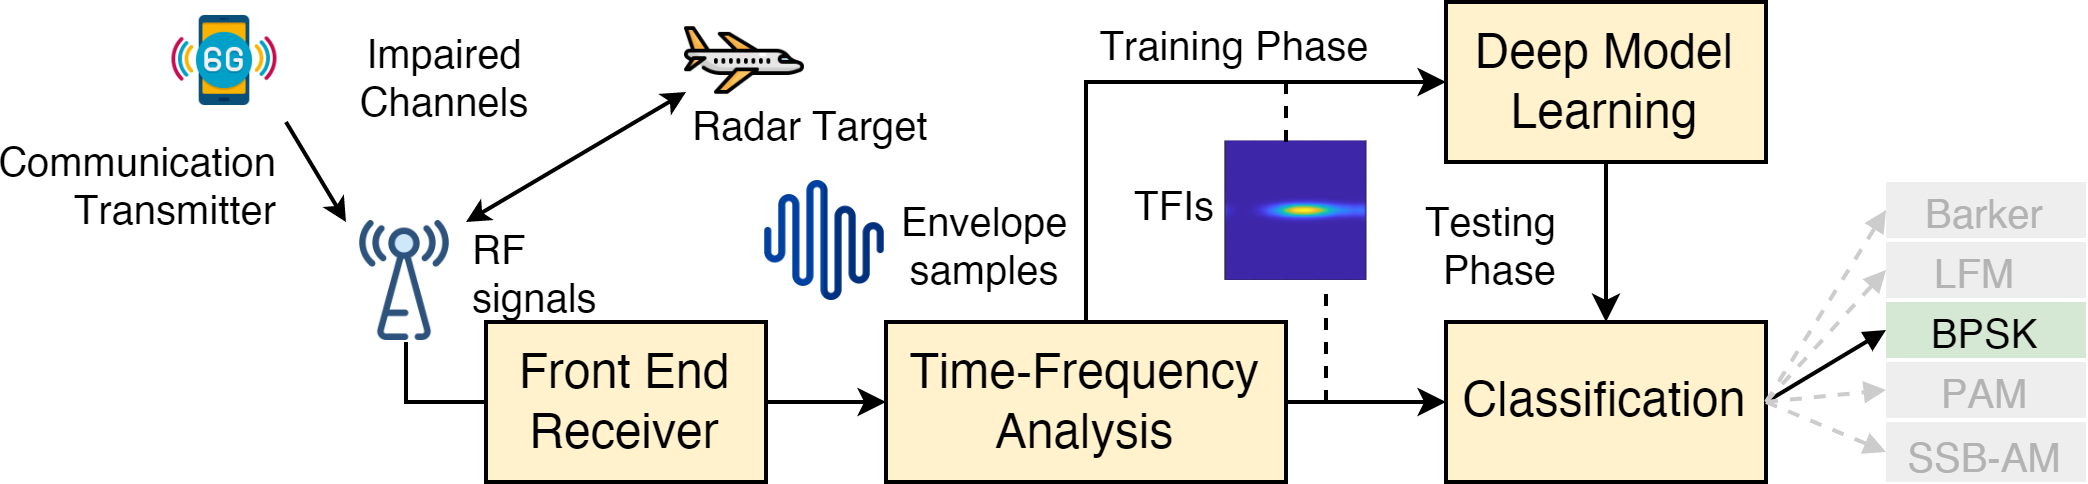
\includegraphics[width=14cm]{fig/fig01.png}    % hình được lưu trong thư mục fig (menu bên trái)
	\caption{Caption của hình là ...}
	\label{fig01}
\end{figure}

\subsubsection{Công thức toán học}
Công thức toán học được trình bày và đánh số tự động như trong công thức~(\ref{eqn01})...
\begin{equation}
h\left ( z \right )=\begin{cases}
z & \text{ if } z\geq 0 \\ 
0 & \text{ if } z < 0
\end{cases}.
\label{eqn01}
\end{equation}

\section{Cơ sở dữ liệu}
\subsection{Firebase Realtime Database}
Firebase Realtime Database ...
\subsubsection{Firebase A}
Firebase A là gì ...
\subsubsection{Firebase B}
Firebase B là gì ...
\subsection{Google Sheet}
Google Sheet là gì ...



% tài liệu tham khảo theo chuẩn IEEE
% tài liệu tham khảo được khai báo trong file refs.bib
\bibliographystyle{IEEEtran} % ieeetr
\bibliography{refs}

\end{document}
